\section{Computations}
\label{sec:results}

This section reports the computations behind the statements of \Cref{sec:theory} and the two enumerative results of the paper.
All counts and all swap gaps were computed in exact integer or rational arithmetic; Monte Carlo results are reported with standard errors.
Hardware, software and algorithms are described in \Cref{sec:appendix}.

\subsection{Exhaustive enumeration for $n=3$}
\label{sec:n3_exhaustive}

All $9!=362{,}880$ arrangements of order $3$ were enumerated in exact integer arithmetic.
Exactly $8$ arrangements have $\Efull=0$ (the Lo Shu orbit), and the same $8$ are the zeros of $\Elow$ (\Cref{rem:n3_lowmode});
$760$ arrangements satisfy the degree-one conditions, $4{,}224$ have both diagonals summing to $15$, and $72$ are semi-magic.
Both energies have mean $40/27$ (the coincidence is special to $n=3$: $\Var(X)=\frac{n^2-1}{12}$ equals $n\Var(C_j)=\frac{n-1}{n}$
only there), with standard deviations $0.4266$ ($\Efull$) and $0.8370$ ($\Elow$), modes $138/81$ and $90/81$, maxima
$180/81$ and $360/81$, and $177$ and $346$ distinct values, all multiples of $1/81$.
Under single swaps the symmetric $\Efull$ has $16$ local minima, the $8$ magic squares and $8$ non-magic arrangements at
$\Efull=2/81$ (two line deviations of $\pm1$); $\Elow$ is more rugged, with $344$ local minima, $336$ of them non-magic.

\subsection{The energy of a random arrangement}
\label{sec:random_energy}

Let $S$ be a uniformly random arrangement, i.e.\ the values $1,\dots,N$ are placed in the
grid by a uniformly random permutation $\pi$. For a test function $\varphi$ on the grid write
$T_\varphi := \Cov(\varphi,Z) = \sum_{c} a_c\, z_{\pi(c)}$ with $a_c=(\varphi_c-\bar\varphi)/N$;
this is a linear permutation statistic in the sense of \Cref{sec:bg_perm}, and its first two moments
follow from \eqref{eq:ww_identity}. Throughout, $\Var(\varphi)$ and $\Cov(\varphi,\psi)$ denote
population variances and covariances over the $N$ cells, and
\[
\sigma_n^2 := \frac{\Var(Z)}{N-1} = \frac{N+1}{12} = \frac{n^2+1}{12},
\qquad \Var(Z)=\frac{N^2-1}{12}.
\]

\begin{proposition}[Exact moments of the random energies]
\label{prop:random_energy_moments}
For a uniformly random arrangement and any test functions $\varphi,\psi$,
\begin{equation}
\E[T_\varphi]=0,\qquad
\E[T_\varphi T_\psi] = \sigma_n^2\,\Cov(\varphi,\psi).
\label{eq:cov_T}
\end{equation}
Consequently, with $\Elow$ as in \eqref{eq:Elow} and the symmetric
$\Efull$ (all $n$ rows, all $n$ columns, both diagonals; $2n+2$ terms),
\begin{align}
\E\,\Cov(X,Z)^2 &= \E\,\Cov(Y,Z)^2 = \frac{n^4-1}{144},\qquad
\E\,\Cov(D,Z)^2 = \E\,\Cov(R_k,Z)^2 = \frac{(n-1)(n^2+1)}{12\,n^2},
\label{eq:single_terms}\\
\E[\Elow] &= \frac{(n^2+1)\,(n^4-n^2+12n-12)}{72\,n^2}
= \frac{n^4}{72}+\frac{n}{6}-\frac{13}{72}+\frac{1}{6n}-\frac{1}{6n^2},
\label{eq:mean_low}\\
\E[\Efull] &= \frac{n^4-1}{6\,n^2} = \frac{n^2}{6}-\frac{1}{6n^2}.
\label{eq:mean_full}
\end{align}
The covariance matrix $\Sigma_n:=\sigma_n^2 G$ of the vector of covariances is $\sigma_n^2$ times
the Gram matrix $G$ of the centred test functions. For $\Elow$,
$G=\operatorname{diag}\!\big(\tfrac{n^2-1}{12},\tfrac{n^2-1}{12},\tfrac{n-1}{n^2},\tfrac{n-1}{n^2}\big)$
except that the two diagonal indicators have $\Cov(D_{\mathrm{m}},D_{\mathrm{a}})=-1/n^2$ when
$n$ is even (they are uncorrelated when $n$ is odd). For $\Efull$, $G$ is block diagonal:
the $n$ row indicators have Gram block $\tfrac1n(I-\tfrac1n J)$, the columns likewise, every
row--column, row--diagonal and column--diagonal covariance vanishes, and the diagonal block is as for
$\Elow$. Hence the eigenvalues of $\Sigma_n$ are
\begin{equation}
\Elow:\ \sigma_n^2\Big\{\tfrac{n^2-1}{12}\,(\times 2),\ \tfrac{n-1}{n^2}\,(\times 2)\Big\},
\qquad
\Efull:\ \sigma_n^2\Big\{\tfrac1n\,(\times\,2n-2),\ \tfrac{n-1}{n^2}\,(\times 2)\Big\}
\label{eq:weights}
\end{equation}
for odd $n$; for even $n$ the last pair $\{\tfrac{n-1}{n^2},\tfrac{n-1}{n^2}\}$ is replaced by
$\{\tfrac1n,\tfrac{n-2}{n^2}\}$. Finally, the variances are explicit rational functions of $n$, given as
\eqref{eq:var_low} in \Cref{sec:app_variance}, with $\Var(\Elow)=n^8/5184+O(n^7)$ and $\Var(\Efull)=n^3/36+O(n^2)$.
\end{proposition}

\begin{proof}
Since $\sum_c a_c=0$, $\E[T_\varphi]=\bar z\sum_c a_c=0$. For two linear permutation
statistics $T_a=\sum_i a_i b_{\pi(i)}$, $T_{a'}=\sum_i a'_i b_{\pi(i)}$ the classical identity
\eqref{eq:ww_identity} reads
$\Cov(T_a,T_{a'})=\frac{1}{N-1}\sum_i(a_i-\bar a)(a'_i-\bar a')\sum_j(b_j-\bar b)^2$.
With $a=(\varphi-\bar\varphi)/N$, $a'=(\psi-\bar\psi)/N$, $b=z$ this is
$\frac{1}{N-1}\cdot\frac{N\Cov(\varphi,\psi)}{N^2}\cdot N\Var(Z)=\sigma_n^2\Cov(\varphi,\psi)$,
which is \eqref{eq:cov_T}. The entries of $G$ are elementary: $\Var(X)=\Var(Y)=\frac{n^2-1}{12}$; a line
indicator has $\Var(L)=\frac1n(1-\frac1n)$; two lines meeting in $m$ cells have $\Cov(L,L')=\frac{m}{N}-\frac{1}{n^2}$
(\Cref{lem:W_structure}); and $\Cov(X,Y)=0$, $\Cov(X,D)=\Cov(Y,D)=0$ since a diagonal contains every column and every row
coordinate exactly once.  Taking traces of $\Sigma_n$ gives \eqref{eq:single_terms}--\eqref{eq:mean_full}:
$\E[\Elow]=\sigma_n^2\big(2\cdot\frac{n^2-1}{12}+2\cdot\frac{n-1}{n^2}\big)$ and
$\E[\Efull]=\sigma_n^2(2n+2)\frac{n-1}{n^2}$. The eigenvalues
\eqref{eq:weights} follow from the block structure, $\tfrac1n(I-\tfrac1nJ)$ having eigenvalue
$\tfrac1n$ with multiplicity $n-1$ and $0$ once.

The variances are obtained by expanding $\E[E^2]$ over the equality patterns of cell quadruples and
using the exact fourth moments of a uniform permutation (\Cref{sec:appendix}); the result is a rational number
for each $n$, and the closed forms \eqref{eq:var_low} were obtained by exact rational interpolation on
$n=3,\dots,45$, verified on $5$--$11$ further orders each and against the exhaustive $n=3$ values
$\Var(\Elow)=1532/2187$, $\Var(\Efull)=398/2187$.
\end{proof}

\begin{corollary}[Limiting law]
\label{cor:random_energy_clt}
As $n\to\infty$, the standardised vector
\[
\bigl(T_X/\sqrt{\Sigma_{11}},\ T_Y/\sqrt{\Sigma_{22}},\ T_{D_{\mathrm{m}}}/\sqrt{\Sigma_{33}},\ T_{D_{\mathrm{a}}}/\sqrt{\Sigma_{44}}\bigr)
\]
converges in distribution to a standard Gaussian vector in $\R^4$, and therefore
\begin{equation}
\frac{\Elow}{(n^4-1)/144}\ \xrightarrow{\ d\ }\ \chi^2_2,
\qquad\text{equivalently}\qquad
\frac{\Elow}{\E[\Elow]}\ \xrightarrow{\ d\ }\ \mathrm{Exp}(1).
\label{eq:low_limit}
\end{equation}
For finite $n$ the Gaussian approximation gives $E\approx\sum_j w_j\chi^2_{1,j}$ with independent
$\chi^2_1$ variables and weights $w_j$ the eigenvalues \eqref{eq:weights}; its density is computed by
Imhof's inversion formula \cite{imhof1961} in Figure~\ref{fig:random_energy}.
\end{corollary}

\begin{proof}
Each fixed linear combination $\sum_k\alpha_kT_{\varphi_k}$ is again a linear permutation statistic $\sum_c a_c z_{\pi(c)}$.
Hoeffding's theorem \cite[Thm.~3]{hoeffding1951} (\Cref{sec:bg_perm}) asserts asymptotic normality provided that, for every
$r\ge3$, $N^{-1}\sum_{i,j}|d_N(i,j)|^r$ is $O\bigl((N^{-1}\sum_{i,j}d_N(i,j)^2)^{r/2}\bigr)$, $d_N$ the doubly centred array.
In the product case $c_N(i,j)=a_iz_j$ the ratio of the two sides equals $N^{1-r/2}\kappa_r(a)\kappa_r(z)$ with $\kappa_r$ the
standardised $r$-th absolute moments.  For $z$ (uniform on $\{1,\dots,N\}$, centred) $\kappa_r(z)=O(1)$; for each of $X$, $Y$
and the two diagonal indicators, $\kappa_r(a)=O(n^{r/2-1})=O(N^{r/4-1/2})$ (the worst case is an indicator of $n$ of the
$N$ cells, a Bernoulli$(1/n)$ variable), so the ratio is $O(N^{1/2-r/4})\to0$.  The same bound holds for every fixed
combination $a=\sum_k\alpha_ka_k$ of the four standardised test functions: $\|a\|_r\le\sum_k|\alpha_k|\|a_k\|_r$ by
Minkowski's inequality, while $\Var(\sum_k\alpha_kT_k)\ge(1-o(1))\sum_k\alpha_k^2$ because the only nonzero correlation among
the $T_k$ tends to zero.  By the Cram\'er--Wold device the vector is asymptotically Gaussian with covariance $\Sigma_n$; for
even $n$ the only nonzero correlation is $\operatorname{corr}(T_{D_{\mathrm{m}}},T_{D_{\mathrm{a}}})=-1/(n-1)\to0$, so the
standardised limit is $N(0,I_4)$.  In $\Elow=\Sigma_{11}(\tilde T_X^2+\tilde T_Y^2)+\Sigma_{33}\tilde T_{D_m}^2+\Sigma_{44}\tilde T_{D_a}^2$
the diagonal terms carry weight $\Sigma_{33}/\Sigma_{11}=12(n-1)/(n^2(n^2-1))\to0$, giving \eqref{eq:low_limit}; the second
form uses $\E[\Elow]/((n^4-1)/72)\to1$.
\end{proof}

\begin{remark}
For $\Efull$ the number of statistics grows with $n$, so the corollary does not apply verbatim; the Gaussian mixture
$\sigma_n^2\big[\tfrac1n\chi^2_{2n-2}+\tfrac{n-1}{n^2}\chi^2_2\big]$ is only a heuristic at the orders we can simulate, and the
ratio of the exact to the Gaussian-mixture variance is $0.24, 0.45, 0.56, 0.64, 0.69, 0.73$ for $n=3,\dots,8$ (for $\Elow$:
$0.51, 0.76, 0.86, 0.90, 0.93, 0.95$).  For $n=3$, $\Elow$ takes $346$ and $\Efull$ $177$ distinct values, all multiples
of $1/81$; the Kolmogorov distances $0.10$ and $0.20$ at $n=3$ are inflated by this discreteness and are not a failure of the
Gaussian approximation as such.
\end{remark}

\begin{table}[htbp]
\centering
\small
\begin{tabular}{c l r r r r r r r}
\toprule
$n$ & energy & $\E[E]$ exact & MC mean & $\sqrt{\Var E}$ exact & MC std & Gauss.\ std & $|\delta_{\mathrm{mean}}|$ & KS \\
\midrule
3 & $\Elow$  & $40/27=1.4815$ & 1.4814 & 0.8370 & 0.8369 & 1.171 & $6\times10^{-5}$ & 0.103 \\
3 & $\Efull$ & $40/27=1.4815$ & 1.4815 & 0.4266 & 0.4266 & 0.869 & $8\times10^{-6}$ & 0.200 \\
4 & $\Elow$  & $391/96=4.0729$ & 4.0736 & 3.1284 & 3.1288 & 3.586 & $2\times10^{-4}$ & 0.037 \\
4 & $\Efull$ & $85/32=2.6562$ & 2.6564 & 0.9074 & 0.9073 & 1.349 & $7\times10^{-5}$ & 0.107 \\
5 & $\Elow$  & $234/25=9.3600$ & 9.3605 & 8.0483 & 8.0482 & 8.694 & $6\times10^{-5}$ & 0.019 \\
5 & $\Efull$ & $104/25=4.1600$ & 4.1600 & 1.3966 & 1.3966 & 1.867 & $9\times10^{-6}$ & 0.078 \\
6 & $\Elow$  & $2035/108=18.843$ & 18.843 & 17.122 & 17.122 & 18.007 & $4\times10^{-5}$ & 0.012 \\
6 & $\Efull$ & $1295/216=5.9954$ & 5.9957 & 1.9671 & 1.9671 & 2.459 & $6\times10^{-5}$ & 0.061 \\
7 & $\Elow$  & $5050/147=34.354$ & 34.349 & 32.174 & 32.167 & 33.349 & $1\times10^{-4}$ & 0.008 \\
7 & $\Efull$ & $400/49=8.1633$ & 8.1631 & 2.5697 & 2.5698 & 3.089 & $2\times10^{-5}$ & 0.050 \\
8 & $\Elow$  & $22295/384=58.060$ & 58.058 & 55.377 & 55.381 & 56.888 & $3\times10^{-5}$ & 0.007 \\
8 & $\Efull$ & $1365/128=10.664$ & 10.664 & 3.2352 & 3.2353 & 3.777 & $3\times10^{-5}$ & 0.042 \\
\bottomrule
\end{tabular}
\caption{Exact moments of Proposition~\ref{prop:random_energy_moments} against Monte Carlo
($10^8$ uniformly random arrangements per order; for $n=3$ the exact values were also confirmed by
enumerating all $9!$ arrangements). $|\delta_{\mathrm{mean}}|$ is the relative error of the MC mean;
all MC means and variances agree with the exact values to within $5\times10^{-4}$ relative error,
consistent with the sampling standard errors. ``Gauss.\ std'' is the standard deviation
of the Gaussian-limit mixture $\sum_j w_j\chi^2_1$ of Corollary~\ref{cor:random_energy_clt}, and KS
is the Kolmogorov distance between the MC sample and that mixture (not the Exp(1) limit).}
\label{tab:random_energy}
\end{table}

\begin{figure}[htbp]
\centering
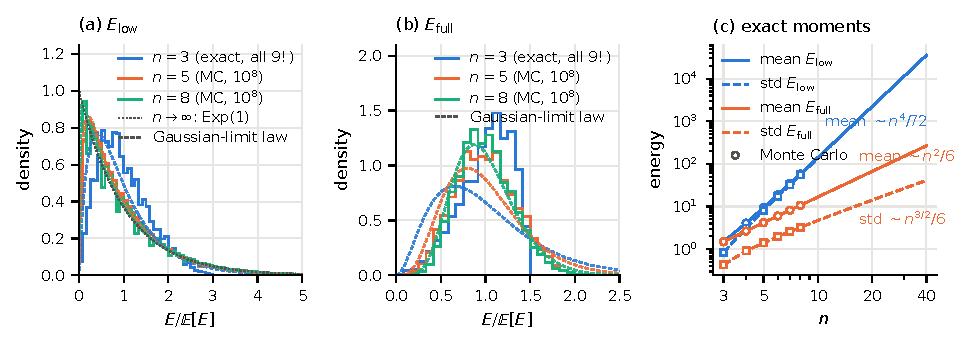
\includegraphics[width=0.92\textwidth]{figures/fig_random_energy.pdf}
\caption{Energy of a uniformly random arrangement. (a) Distribution of
$\Elow/\E[\Elow]$ for $n=3$ (exact, all $9!$ arrangements) and
$n=5,8$ ($10^8$ Monte Carlo samples each), with the Gaussian-limit mixture densities (dashed, Imhof
inversion with the weights \eqref{eq:weights}) and the $n\to\infty$ limit $\mathrm{Exp}(1)$ of
Corollary~\ref{cor:random_energy_clt} (dotted). (b) The same for the symmetric $\Efull$;
here the Gaussian mixture is only a slowly improving approximation (see the remark after
Corollary~\ref{cor:random_energy_clt}). (c) Exact mean (solid) and standard deviation (dashed) of
both energies from Proposition~\ref{prop:random_energy_moments}, $3\le n\le 40$, with the Monte Carlo
values for $n=3,\dots,8$ (open markers). The mean of $\Elow$ grows like $n^4/72$ and its
standard deviation like $n^4/72$ as well (an exponential limit has unit coefficient of variation);
$\Efull$ has mean $\sim n^2/6$ and standard deviation $\sim n^{3/2}/6$.}
\label{fig:random_energy}
\end{figure}

\subsection{Swap gaps: exact verification}
\label{sec:swap-gaps}

\Cref{thm:swap} gives, for a magic square $S$ and the swap of two cells $a,b$ with $d=|s_a-s_b|$,
$\Efull(S^{ab})=d^{2}m(a,b)/N^{2}$ with $m(a,b)\in\{2,\dots,6\}$ the number of lines separating $a$ from $b$.
We verified the formula in exact rational arithmetic, with the symmetric energy evaluated directly from the definition, on
every one of the $880\cdot\binom{16}{2}=105{,}600$ single swaps of the $880$ essentially different order-$4$ squares, the
$8\cdot\binom92=288$ swaps of the eight order-$3$ squares, and all swaps of the Siamese squares of orders $5$, $7$ and $9$:
agreement in every case, and $\Efull(S)=0$ exactly for every magic square.  The gap spectrum is arithmetic, not ``banded'':
over the $105{,}600$ order-$4$ swaps $N^2\Delta E=d^2m$ takes exactly $70$ distinct integer values from $2$ to
$980=14^2\cdot5$, and the minimum gap $N^2\Delta_{\min}(S)$ is $2$ for $432$ squares, $3$ for $420$ and $4$ for $28$
(\Cref{cor:local_min}(3)); it is $3$ for all eight order-$3$ squares and $3$, $2$, $2$ for the Siamese squares of orders
$5$, $7$, $9$.

% ===========================================================================

\subsection{The low-mode balanced class for $n=4$}
\label{sec:lowmode_n4}

Write $L_n$ for the set of arrangements of $\{1,\dots,N\}$ with
$\Cov(X,Z)=\Cov(Y,Z)=\Cov(D_{\mathrm{m}},Z)=\Cov(D_{\mathrm{a}},Z)=0$,
i.e.\ $\Elow=0$ (\Cref{cor:Elow_degree1}).  Each of the four conditions is a \emph{linear} statistic of the
arrangement: with cells indexed by $(i,j)\in\{0,\dots,n-1\}^2$,
$\Cov(X,Z)=0 \iff T_1:=\sum_{i,j} j\,s_{ij} = \tfrac{n-1}{2}\cdot\tfrac{N(N+1)}{2}$,
$\Cov(Y,Z)=0 \iff T_2:=\sum_{i,j} i\,s_{ij}$ equals the same target, and the two diagonal
conditions say that $T_3=\sum_i s_{ii}$ and $T_4=\sum_i s_{i,n-1-i}$ equal $M(n)=n(N+1)/2$.

\begin{proposition}[Exact size of $L_4$]
\label{prop:L4}
$|L_3| = 8$ (the Lo Shu orbit; the class with only $\Cov(X,Z)=\Cov(Y,Z)=0$ has $760$ members), and
\[
  |L_4| \;=\; 14\,639\,440 \;=\; 8\times 1\,829\,930 ,
\]
of which exactly $7040$ are magic squares.  The class is $D_4$-invariant and $D_4$ acts freely on it
($1\,829\,930$ orbits of size $8$).  The first-moment class
$\{\Cov(X,Z)=\Cov(Y,Z)=0\}$ has $6\,697\,177\,424$ members for $n=4$,
and the class with both diagonals equal to $34$ has $49\,932\,288\,000$ members.
\end{proposition}

\begin{proof}[Computation]
The count is a meet-in-the-middle enumeration over the four additive statistics $T_1,\dots,T_4$ (\Cref{sec:appendix}; $9$\,s on
$16$ threads), with the matching pairs expanded explicitly to obtain the row- and column-sum breakdown of \Cref{tab:L4}.
Validation: on $n=3$ the same program reproduces the brute-force counts $8$, $760$, $4224$, $8$ magic and $72$ semi-magic; on
$n=4$, with the $2n$ line sums in place of $T_1,T_2$, it reproduces the $7040$ magic and the $549{,}504=8\times68{,}688$
semi-magic squares; the diagonal-only count was also obtained by direct combinatorics, and the probability $|L_4|/16!$ was
checked by $2\times10^{9}$ Monte Carlo samples ($1373$ hits; relative error $2.7\%$).
\end{proof}


\begin{table}[H]
\centering
\caption{Breakdown of $L_4$ by the number of row sums and column sums equal to $M(4)=34$.
Exactly two or three equal row sums are impossible: if $R_i=34+e_i$ then $\sum_i e_i=0$ and
$\sum_i i\,e_i=0$ (this is $T_2$), which cannot hold with exactly one or two nonzero $e_i$;
the same holds for columns.  The table is symmetric under transposition.}
\label{tab:L4}
\begin{tabular}{lrrrr}
\toprule
 & \multicolumn{4}{c}{columns equal to 34} \\
\cmidrule(lr){2-5}
rows equal to 34 & 0 & 1 & 4 & total \\
\midrule
0 & 9\,637\,312 & 2\,172\,824 & 100\,728 & 11\,910\,864 \\
1 & 2\,172\,824 & 429\,312 & 9\,336 & 2\,611\,472 \\
4 & 100\,728 & 9\,336 & \textbf{7\,040} (magic) & 117\,104 \\
\midrule
total & 11\,910\,864 & 2\,611\,472 & 117\,104 & 14\,639\,440 \\
\bottomrule
\end{tabular}
\end{table}

Thus only $7040/14\,639\,440 = 0.048\%$ of the low-mode balanced arrangements are magic;
$110\,064$ members have all row sums equal to 34 but not all column sums (and symmetrically),
and $9\,637\,312$ (66\%) have \emph{no} row or column summing to $34$ at all; the arrangement
of \Cref{rem:four_term_insufficient} belongs to the last class.

\paragraph{Why random sampling never found a counterexample.}
$|L_4|/16! = 6.997\times10^{-7}$, about one arrangement in $1.43$ million, so the estimate ``below $10^{-8}$'' given in the
previous version of this paper was too small by a factor of about $70$.  The $10^8$-sample runs of \Cref{sec:random_energy}
contain $61$ members of $L_4$, against an expectation of $70.0\pm8.4$ ($1.1$ standard deviations low).  The previous version
reported that $6\times10^7$ samples for $n=4$ contained no member of $L_4$, a $42$-fold shortfall.  On re-examination, the
archived data file behind that statement holds $10^5$ samples per order (the script's default), for which the expected number
of members is $0.07$, and we found no record of a larger run; the two other candidate causes are excluded (the energy evaluated
by that code has the same zero set as $\Elow$, and it evaluates to an exact floating-point zero on members of $L_4$, so no
tolerance could have missed them).  We attribute the earlier statement to a misreported sample size, but the cause cannot be
reconstructed from the repository.
A Gaussian local-limit estimate explains the order of magnitude of $|L_4|$: under a uniformly random arrangement the vector
$(T_1,\dots,T_4)$ has mean equal to the target vector (by symmetry) and covariance $\Sigma$ given by \eqref{eq:ww_identity} ($T_1,T_2$ are uncorrelated with each other and with the
diagonals; the two diagonal sums have correlation $-1/(n-1)$ for even $n$ and $0$ for odd $n$), and the $\Z$-span of the
change vectors of all single transpositions has index $1$ in $\Z^4$ (Smith normal form, computed for $n\le8$), so
\[
  |L_n| \;\approx\; N!\,(2\pi)^{-2}\det(\Sigma)^{-1/2}.
\]
The estimate gives $13.6$ for $n=3$ (true: $8$, ratio $0.59$) and $1.82\times10^{7}$ for $n=4$ (true:
$14\,639\,440$, ratio $0.80$); for the two-condition classes the ratios are $0.59/0.91$ (first moments)
and $1.10/0.96$ (diagonals), so the Gaussian approximation improves with $n$ as the local limit theorem
predicts.  For $n=5,6$ we have no exact count; the estimate gives $6.7\times10^{17}$ and $1.5\times10^{33}$, and Monte Carlo
($10^{10}$ and $2\times10^{10}$ samples) gives $5.1\times10^{17}$ ($\pm6\%$) and $1.2\times10^{33}$ ($\pm13\%$), conjectural
orders of magnitude only.
In every case the magic squares are a vanishing fraction of $L_n$: the four low-mode conditions cost a factor of order
$\det(\Sigma)^{1/2}\propto n^{13}$, while a magic square requires $2n$ independent line conditions, each costing a further
factor of order $n^{5/2}$.


\subsection{Geometry of the 880 order-4 gems}
\label{sec:gem-geometry-880}

For each of the $880$ essentially different order-$4$ magic squares we computed the Magic Gem $\mathcal G(S)$ exactly
(integer facet planes, merged coplanar triangles, rational volumes; \Cref{sec:appendix}); Euler's relation holds for all
$880$ gems.  \Cref{fig:gem-geometry-880} and \Cref{tab:gem-fvectors} summarise the results.

\begin{table}[htbp]
\centering
\caption{Face structure of the $880$ order-$4$ gems by number of hull vertices $V$: number of squares, of distinct
combinatorial types (face lattices up to isomorphism), of distinct exact volumes, and of distinct $f$-vectors $(V,E,F)$.
The full list of the $39$ $f$-vectors with multiplicities is in the ancillary file \texttt{revision\_round2/appendix\_data.json}.}
\label{tab:gem-fvectors}
\small
\begin{tabular}{r rrrrrrrrr r}
\toprule
$V$ & 8 & 9 & 10 & 11 & 12 & 13 & 14 & 15 & 16 & all\\
\midrule
squares & 7 & 10 & 103 & 80 & 380 & 106 & 162 & 14 & 18 & 880\\
types   & 4 & 1 & 27 & 32 & 129 & 52 & 85 & 7 & 15 & 352\\
volumes & 4 & 5 & 51 & 33 & 111 & 40 & 65 & 6 & 14 & 155\\
$f$-vectors & 4 & 1 & 6 & 5 & 7 & 5 & 5 & 3 & 3 & 39\\
\bottomrule
\end{tabular}
\end{table}

\paragraph{Vertex counts, $f$-vectors, volumes.}
Between $8$ and all $16$ of the points are hull vertices; $V=12$ is modal ($380/880$).  There are $39$ distinct $f$-vectors,
from $(8,14,8)$ (one gem, square \#54) and $(8,16,10)$ (one gem) to $(16,36,22)$ (nine gems), the modal one being
$(12,26,16)$ ($164$ gems); the multiset of facet sizes (number of triangles, quadrilaterals, \dots) is determined by the
$f$-vector in every case.  The exact volume takes $155$ distinct values, from
$58$ (square \#427) to $292/3$ (square \#379), mean $84.05$.  The denominators are $1,2,3,6$: all three
coordinates of every point are half-odd integers when $n$ is even, so the translate of a gem by $(\frac12,\frac12,\frac12)$ is a
lattice polytope of $\Z^3$ and its volume lies in $\frac16\Z$.
Surface areas range from $116.5$ to $148.6$.

\paragraph{Combinatorial types.}
Two gems have the same combinatorial type if their vertex--facet incidence
structures (equivalently, their face lattices) are isomorphic.  Grouping by a
Weisfeiler--Lehman hash of the bipartite vertex--facet graph and confirming
every group by an explicit graph isomorphism test gives
\[
352\ \text{combinatorial types}
\]
among the $880$ gems (the hash was already exact: no hash class had to be
split).  Their sizes are very uneven; the number of types with $1,2,3,\dots$ members is
\[
\begin{array}{r|rrrrrrrrrrrrrr}
\text{squares per type} & 1&2&3&4&5&6&7&8&10&13&14&16&26&32\\\hline
\text{types} & 93&201&8&20&4&7&4&5&5&1&1&1&1&1
\end{array}
\]
(\Cref{fig:gem-geometry-880}c); the largest type, with $f=(10,22,14)$ (12 triangles,
2 quadrilaterals), is shared by $32$ squares, and the second largest,
$f=(12,24,14)$, by $26$.  The $7$ gems with $8$ vertices fall into $4$ types,
including a single $(8,14,8)$ gem with four triangular and four quadrilateral
faces (square \#54, Fig.~\ref{fig:gem-geometry-880}d) and four
$(8,18,12)$ gems sharing one simplicial type with $12$ triangular faces.  The $18$ gems with all $16$ points
extreme belong to $15$ types.

\paragraph{Congruence classes and injectivity.}
Two gems are \emph{congruent} if an isometry of $\mathbb R^3$ (rotations, reflections, translations) maps one onto the
other; since a distance-preserving bijection between finite point sets extends to an isometry, congruence is decided exactly
by testing for a bijection of hull-vertex sets preserving all integer squared distances (\Cref{sec:appendix}).

\begin{proposition}[class $\to$ gem]
\label{prop:gem-injective}
\begin{enumerate}
\item The $880$ hull-vertex sets are pairwise distinct: the map from
  $D_4$-classes of order-$4$ magic squares to hull-vertex sets (as subsets of
  $\mathbb R^3$) is injective.  (For the full $16$-point sets this is trivial, since the point set determines the
  arrangement.)
\item Up to congruence there are exactly $616$ gems.  The congruence classes
  are precisely the orbits of the complement map $S\mapsto 17-S$, which acts
  on gems as the reflection $z\mapsto -z$: $352$ squares are
  self-complementary (their gems are mirror-symmetric up to a lattice
  symmetry) and the other $528$ form $264$ mirror pairs.  No two gems of
  non-complementary squares are congruent, not even as full $16$-point sets.
\end{enumerate}
\end{proposition}

Part (2) is the only failure of injectivity, and it is the expected one: $17-S$ is magic whenever $S$ is, and its gem is the
mirror image of $\mathcal G(S)$ in the plane $z=0$.  The $352$ self-complementary classes are exactly Dudeney's group III (the
$48$ associated squares) together with all $304$ squares of group VI \cite{dudeney1917amusements}.  The coincidence
$352=\#\{\text{types}\}=\#\{\text{self-complementary squares}\}$ is numerical only: the two partitions of the $880$ are different.

\paragraph{Dudeney groups.}
Crossing the hull-vertex count with Dudeney's twelve groups (table in the ancillary files) shows that geometry is only
loosely tied to Dudeney type: every group with more than eight members spans at least four vertex counts and at least $20$
combinatorial types; the $8$-vertex gems occur only in groups VI (three) and VIII (four).


\begin{remark}
Groups III and VI, the self-complementary ones, have only even vertex counts;
this is forced: for a self-complementary square the reflection $z\mapsto-z$
composed with the element of $D_4$ that realises $17-S$ is an isometry of
the gem of order $2$ or $4$ without fixed hull vertices (no point has $z=0$
when $N$ is even), so hull vertices fall into orbits of size $2$ or $4$.
\end{remark}

\begin{figure}[htbp]
\centering
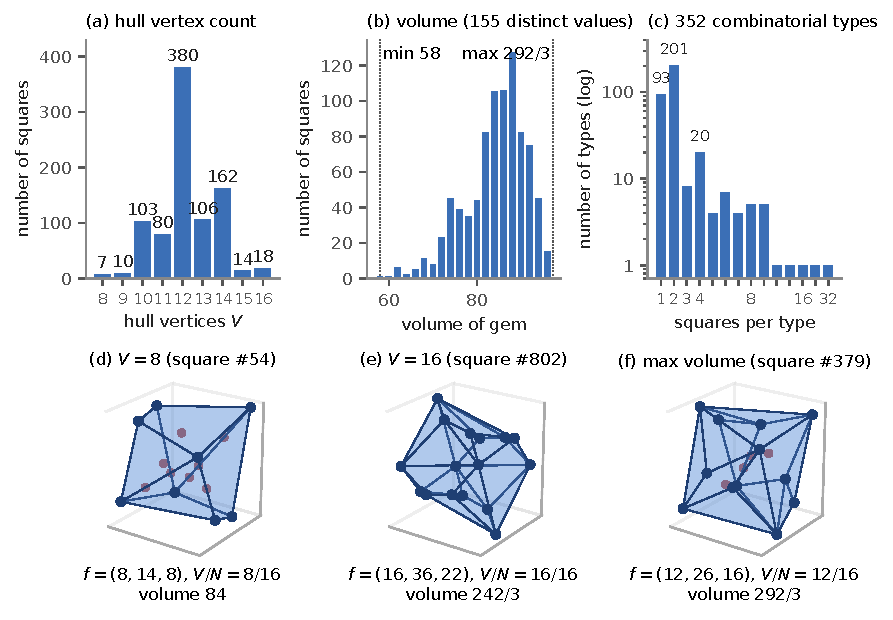
\includegraphics[width=0.9\textwidth]{figures/fig_gem_geometry_880.pdf}
\caption{Geometry of the $880$ order-$4$ Magic Gems.
(a)~Number of hull vertices ($8$ to $16$; modal value $12$).
(b)~Exact hull volume ($155$ distinct values between $58$ and $292/3$).
(c)~Sizes of the $352$ combinatorial types (logarithmic scale): $93$ types occur once, $201$
twice, and one type is shared by $32$ squares.
(d)--(f)~Three extreme gems, drawn with translucent faces after merging
coplanar triangles: the unique $(8,14,8)$ gem (square \#54; the eight
interior points are shown in red), a gem with all $16$ points extreme
(square \#802, D\"urer's square with its first two rows exchanged and its last two rows exchanged), and the gem of largest
volume (square \#379).}
\label{fig:gem-geometry-880}
\end{figure}

\paragraph{Named squares.}
The gems of the Lo Shu, of D\"urer's square and of the Siamese square of order $5$ have hull fractions $8/9$, $12/16$ and
$12/25$ and exact volumes $18$, $92$ and $830/3$.  D\"urer's own gem has twelve vertices, but exchanging its first two rows and
its last two rows (which preserves the magic property) gives a square whose gem has all sixteen points extreme (square \#802,
\Cref{fig:gem-geometry-880}e): the hull-vertex count is a property of the square, not of the Dudeney group or of the
construction method.

% ===========================================================================
\subsection{Siamese gems have twelve vertices}
\label{sec:siamese-gems}

For the Siamese (de la Loub\`ere) squares of odd order the hull-vertex count
does not grow with $n$.  We computed the gems for $n=3,5,\dots,21$: the Lo Shu
gem has $f=(8,16,10)$, and every Siamese gem with $n\ge5$ has
$f=(12,26,16)$ with $12$ triangular and $4$ quadrilateral facets, so the hull
fraction $12/n^2$ tends to zero.  This is a
theorem, with a short computer-assisted proof.

\begin{proposition}[Siamese gems]
\label{prop:siamese-12}
Let $n=2m+1\ge5$ and let $S$ be the Siamese square of order $n$ ($1$ in the
middle cell of the top row, successive entries one step up and to the right
modulo $n$, one step down when blocked).  Then $\mathcal G(S)$ has exactly $12$
vertices, $26$ edges and $16$ facets ($12$ triangles, $4$ quadrilaterals).
With $0$-indexed cells $(i,j)$ and $c=(n^2+1)/2$, the vertices are the
points over the cells
\[
\begin{array}{lll}
(0,0)\colon c+m+2, & (0,m-1)\colon n^2-1, & (0,m)\colon 1, \\
(0,2m)\colon c+m, & (m-1,0)\colon n^2-m, & (m,0)\colon m+2, \\
(m,2m)\colon n^2-m-1, & (m+1,2m)\colon m+1, & (2m,0)\colon c-m, \\
(2m,m)\colon n^2, & (2m,m+1)\colon 2, & (2m,2m)\colon c-m-2,
\end{array}
\]
i.e.\ the four corners, and on each side of the square the two cells holding
the side's extreme values.  For $n=3$ the same construction gives the Lo Shu
gem, with $8$ vertices (all cells except the centre).
\end{proposition}

\begin{proof}
\emph{Step 1: closed form.}  Write $\langle t\rangle\in\{0,\dots,n-1\}$ for
$t\bmod n$.  We claim $s(i,j)=n\langle i+j-m\rangle+\langle i+2j-2m\rangle+1$.
Indeed, along a run of $n$ consecutive entries the move $(i,j)\to(i-1,j+1)$
fixes $i+j$ and increases $i+2j$ by $1$ modulo $n$, while the ``blocked''
move $(i,j)\to(i+1,j)$ increases both $i+j$ and $i+2j$ by $1$; the entry $1$
sits at $(0,m)$ where both expressions vanish.  Hence by induction the entry
$k$ lies in a cell with $\langle i+j-m\rangle=\lfloor (k-1)/n\rfloor$ and
$\langle i+2j-2m\rangle=\langle k-1\rangle$; since
$(i,j)\mapsto(i+j,\,i+2j)$ is a bijection of $\mathbb Z_n^2$ (determinant
$1$), this determines the cell, which proves the claim.

\emph{Steps 2 and 3 (sketch; details in \Cref{sec:app_siamese}).}  With $m=(n-1)/2$, $x=j-m$, $y=m-i$, the closed form gives
$z=L(x,y)+n\,\zeta(x,y)$ with $L$ affine and
$\zeta=-n\lfloor(x-y+m)/n\rfloor-\lfloor(2x-y+m)/n\rfloor\in\{\pm(n+1),\pm1,0\}$.
The affine bijection $\Phi(x,y,z)=(x,y,(z-L)/n)$ preserves the face lattice and the vertex cells, and
$\Phi(\mathcal G(S))$ is the convex hull of the lattice points of five convex lattice polygons at the five heights $\zeta$:
two triangles $T$, $B=-T$ at $\zeta=\pm(n+1)$, two triangles $U$, $D=-U$ at $\zeta=\pm1$, and a parallelogram $M$ at
$\zeta=0$ (\Cref{fig:siamese-layers}a).  Sixteen explicit planes, eight of them and their images under $(x,y,\zeta)\mapsto
-(x,y,\zeta)$, are shown to support the convex hull of twelve named points $v_1,\dots,v_{12}$---the three corners of $T$ and
of $B$, one corner each of $U$ and $D$, and the four corners of $M$---in facets that close up into a surface with
$(V,E,F)=(12,26,16)$ closed under edge-adjacency, hence all facets (so $P=Q$), and every vertex of every layer polygon satisfies all sixteen inequalities
(\Cref{fig:siamese-layers}b).  These are finitely many polynomial identities and inequalities in $m$, verified exactly for all
integers $m\ge2$ by the script \texttt{siamese\_proof.py}.  Hence $\Phi(\mathcal G(S))=\operatorname{conv}\{v_1,\dots,v_{12}\}$,
and mapping back by $\Phi^{-1}$ gives the statement; for $m=1$ the four triangles degenerate to points and the same argument
gives the $8$-vertex Lo Shu gem.
\end{proof}

\begin{figure}[htbp]
\centering
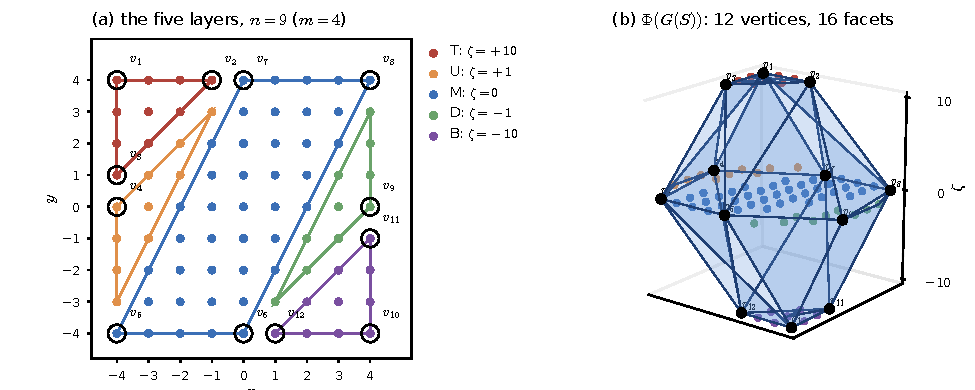
\includegraphics[width=0.88\textwidth]{figures/fig_siamese_layers.pdf}
\caption{The Siamese gem of order $n=9$ after the affine reduction of \Cref{prop:siamese-12}.
(a)~The $81$ cells in the $(x,y)$-plane coloured by the layer value $\zeta\in\{+10,+1,0,-1,-10\}$, with the five lattice
polygons $T,U,M,D,B$ outlined and the twelve vertex cells $v_1,\dots,v_{12}$ circled.
(b)~The reduced polytope $\Phi(\mathcal G(S))=\operatorname{conv}\{(x,y,\zeta)\}$ with its $12$ vertices and $16$ facets
($12$ triangles, $4$ quadrilaterals); the shapes of the layers do not depend on $n$ except through scale, which is why the
combinatorial type is constant for all odd $n\ge5$.}
\label{fig:siamese-layers}
\end{figure}
